%%% Template for the submission to  %%%
%%%     Notre Dame Journal of Formal Logic  (ndjfl)
%%%
%%% Usage summary %%%
%%%     Mostly, the information
%%%     required is obvious, but some explanations are given.
%%%     All other lines should be ignored.  

\documentclass{ndjflart}
%%% HIGHLY RECOMMENDED PACKAGES AND SETTINGS
%\usepackage{pdfsync}  %% if you know what this is use it or not. 
\usepackage[T1]{fontenc}
%%%%%%%%%%%%%%%%%%%%%%%%%%%%%%
%% If your tex system is less than 2 years old (in 2012) the following
%% font options are available. If not comment them out.
\usepackage{tgtermes}
%       otherwise use alternative journal fonts
%\renewcommand{\rmdefault}{ptm} % system default Times font
\usepackage{mathptmx}  
%%%     additional fonts
\usepackage[scaled=.92]{helvet}
%\setoptfont{enc={T1},fam={pop}} % if You have Optima font, uncomment this line
%%% MATH
\usepackage{amsthm,amsmath,amssymb}
\usepackage{mathrsfs}
%%% BIBLIOGRAPHY
\usepackage[numbers]{natbib}  %% numbers is required.
%%% LINKS
\usepackage[colorlinks,citecolor=blue,urlcolor=blue]{hyperref}  %%check
\usepackage{graphicx}

\artstatus{am} %%% leave this alone!!  That means you, too!!
%%%%%%%%theorems%%%%%


%%%% feel free to changes these%%%%%%%
\newtheorem{theorem}{Theorem}[section]
\newtheorem{lemma}[theorem]{Lemma}
\newtheorem{conjecture}[theorem]{Conjecture}
\newtheorem{condition}[theorem]{Condition}
\newtheorem{claim}[theorem]{Claim}
\newtheorem{question}[theorem]{Question}
\newtheorem{corollary}[theorem]{Corollary} 
\theoremstyle{definition}
\newtheorem{definition}[theorem]{Definition}
\newtheorem{statement}[theorem]{Statement}
\newtheorem{notation}[theorem]{Notation} 
\theoremstyle{remark}
\newtheorem{remark}[theorem]{Remark}



%%%DATE enter the date of your submission here- best%%%
%%%If \date{} is not used, the current date will be used%%%
%%%Warning:This will be lost if your paper is recompiled on another day though%%%
%%%\date{May 30, 2012}%%%%
\date{June 22, 2012}

%%%PUT YOUR DEFINITIONS HERE%%%
%NDJFL uses \varphi by default; redefine only if you want \phi%%%

\startlocaldefs
%%% our macros for this article only %%%%
\newcommand{\NDJFL}{\emph{NDJFL}}
\newcommand{\Jo}{\emph{Journal}}
\newcommand{\EM}{Editorial Manager}
\newcommand{\origphi}{\phi}
\newcommand{\CMS}{\emph{CMS}}
\newcommand{\mn}{\medskip\noindent}
\newcommand{\tietilde}{\char126\relax}

\endlocaldefs

\begin{document}

\begin{frontmatter}

  %% TITLE OF YOUR PAPER%%%
  %% Words in title should begin with uppercase, except%%%
  %%% articles (and, the, a), conjunctions (and, for, nor, but),
  %%% prepositions (by, with, for, over, and so on)
  \title{\emph{Style Guide for Submission of Manuscripts to}\\
    \emph{Notre Dame Journal of Formal Logic}}
  %%% Choose a short title to be used as the running head on
  %%% odd-numbered pages%%%
  %%% Use this same title as "short title" when you submit MS to
  %%% EM%%%%
  \runtitle{NDJFL Style Guide}

  \author{\fnms{Martha} %first name
    \snm{Kummerer}%last name
    \corref{}%to denote who is the corresponding author
    \ead[label=e1]{ndjfl@nd.edu}%author email, leave this [label] as is
    \ead[label=u1,url]{http://ndjfl.nd.edu/}%%web page, leave this [label] as is
  }
  %%% ADDRESS NOTES
  %%% Dept listed first, University/company second, street or PO box
  %%% third%%%
  %%% U.S. Postal Service guidelines request no punctuation in the
  %%% street...country lines%%%
  %%% Country should be all uppercase%%%%
  \address{Department of Leisure\\
    University of the World\\
    123 Paradise Lane\\
    Lost Island LI 45678\\
    THE CARIBBEAN\\
    \printead{e1}\\
    \printead{u1} }%
  \and%
  \author{\fnms{Peter}
    \snm{Cholak}\ead[label=e2]{cholak.1@nd.edu}}%increase label by
  %	% one for each
  %	% author
  \address{Department of Mathematics\\
    University of Notre Dame\\
    Notre Dame IN 46556\\
    USA\\
    \printead{e2} }
  % \and \author{\fnms{???} \snm{???}\ead[label=e3]{???}}
  % \address{\printead{e3}} \affiliation{???}

  %%%% INSERT EACH AUTHOR'S FIRST INITIAL AND SURNAME%%%%
  \runauthor{M.~Kummerer and P.~Cholak}


\begin{abstract}
  This document and its \LaTeX\ source are meant as a guide to the
  \emph{Notre Dame Journal of Formal Logic's (NDJFL)} style and the
  style files \emph{ndjflart} and \emph{jflnat.bst}. The files will
  explain the formatting of an article in ndjflart and will address
  the style issues the \Jo\ prefers in the articles it publishes.  The
  abstract should be a very brief summary of the article, that is, no
  more than 150 words. It is lifted from the paper by indexing
  services and therefore should not contain citations to works in the
  \emph{References} nor should it contain author-created macros.
  Limit maths and symbols to those that can be easily converted for
  web reading.  The abstract should be in one block and not separated
  into paragraphs.
\end{abstract}

\begin{keyword}[class=AMS]
  \kwd[Primary ]{X001} \kwd{Y002} \kwd[; Secondary ]{Z003}
\end{keyword}

\begin{keyword}
  \kwd{typesetting} \kwd{guide for authors}
\end{keyword}

\end{frontmatter}

% main matter with bibliography goes here

\section{How Should You Use This Style Guide?}\label{intro}
The \emph{Notre Dame Journal of Formal Logic} welcomes your
submission.  We publish original and significant work in all areas of
logic and the foundations of mathematics.  Your prepared manuscript
will be submitted and processed through
\href{http://www.editorialmanager.com/ndjfl}{Editorial Manager}.
Throughout the review process you can log in at any time and follow
the progress of your manuscript.

This guide will cover the preparation of your manuscript and details
on our particular style.  Our hope is that you will use this style
guide to help you typeset your paper.  No matter which documentclass
you use in composing your paper, you can easily convert it to ndjflart
using the suggestions in the template.  Hopefully this guide will
prove useful whether you are converting a finished document to use
ndjflart.cls, are in the middle of writing the paper, or are just
beginning.

At the very least, this guide describes the \NDJFL\ style. We reserve
the right to edit your paper so it conforms to our style. If you read
this, you will not be surprised when you receive your page proofs.


\begin{figure}
\begin{center}
\vspace{0.5em}
    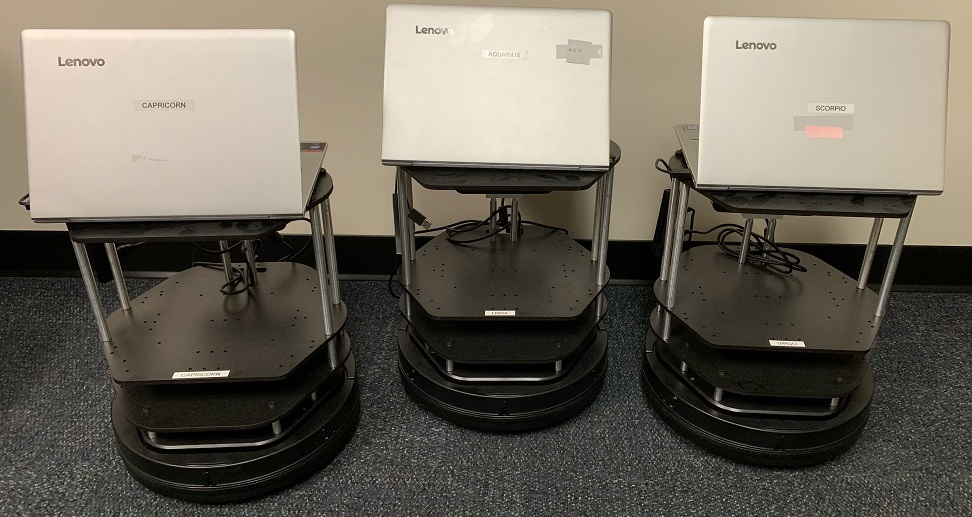
\includegraphics[width=8cm]{images/turtlebots}
    \vspace{-.5em}
\caption{A description of my cool figure. }
\label{fig:framework}
    \end{center}
\end{figure}


\section{Frontmatter}\label{front}
This guide uses the documentclass ``ndjflart'' which you can download
from the\linebreak \href{http://ndjfl.nd.edu}{\NDJFL} website.  It
also requires the artstatus argument ``am'' meaning ``author
manuscript.''  When your paper is typeset, this term will be changed
to incorporate the \Jo's fonts and settings.  You should not change
this.


\subsection{Fonts}\label{fonts} 
Various options appear in the code at the beginning of this template
which you can switch on or off for the fonts available to you.  The
\NDJFL\ uses the MathTime{\tiny\texttrademark} Professional 2
(MTPro2)%
%
\endnote{MathTime{\tiny\texttrademark} Professional 2 (MTPro2) fonts
  are the product of Personal TeX, Inc., San Francisco, CA and
  trademarked by them.}
%
fonts for publishing.  If you have them, you will know how to use them
in this template.

We have available the math alphabets mathcal, mathfrak, mathscr, and
mathbb (e.g., $\mathcal{A}, \mathfrak{A}, \mathscr{A}, \mathbb{A}$).
We use $\varphi$ by default so you do not need to redefine
\verb=\phi=.  However, if you do need this $\origphi$ symbol
throughout your paper, you will need to \verb=\renewcommand=.

%%%% NOTA BENE %%%%%
Developing your own font symbol is \emph{strongly discouraged}.  If
you cannot find a symbol among the standard \LaTeX, amssymb, and
mathrsfs symbols, try the packages stmaryrd, wasy2, or others found at
\href{http://www.ctan.org}{ctan.org}.

Our titles and section headings are in optima font.  Since most users
do not have optima, your system will use helvetica.  When you have
axioms or other items that need a list heading, you can use
\verb=\subsection*= to create a nice flush left heading that will
naturally occur in optima bold when we typeset your paper.  The
following is an example of using this for a list heading.

\subsection*{List of Our Axioms}

\begin{tabbing}
  A1\quad \= ABC\\
  A2\> DEF
\end{tabbing} 

\subsection{Author macros}\label{macros} Load your macros in the
special area between

\mn \verb=\startlocaldefs= and

\mn \verb=\endlocaldefs=.

\mn If you ``input'' a special file containing your macros, be sure to
include it when you are asked for source files upon acceptance of your
paper.

\subsection{Article data}

\subsubsection{Title and runtitle}\label{tandr} The title of your paper should be
printed in headline-style capitalization. In general, this means that
the first and last word and all major words in the title and subtitle
should be uppercase. Articles (an, the, a), conjunctions (and, nor,
or, but), and prepositions (by, with, for, over) should be lowercase.
See \emph{Chicago Manual of Style (CMS)}~\cite{CMS}, especially
Chapter~8.157, ``Principles of headline-style capitalization,'' for
more specific information and exceptional situations such as
hyphenated words.  Keep maths to a minimum in titles.

The \verb=\runtitle= should be your preferred shortened version of
your title.  This is requested when you upload your paper to \EM\ (in
the field called ``short title''). The editors may change this during
the final stages of publishing.  Keep it short; it should not take up
the whole width of the page.  This runtitle will appear on
even-numbered pages.

\subsubsection{Author(s)}\label{authordata} The \verb=\author{}= line
includes the author's name (divided into first name (\verb=\fnms{}=)
with middle initial, if desired, and surname (\verb=\snm{}=) and
e-mail address.  It can also contain a web address, if desired.  A
separate \verb=\author{}= is used for each additional author, but the
\verb=\ead= label is changed to e2,u2 or e3,u3, as appropriate.

On a separate line, the command \verb=\runauthor= contains the data
that will appear as the running head on odd-numbered pages in the
article.  Enter the initial(s) and surname of each author separated by
``and.''  In a series of three or more authors the ``and'' is preceded
by a comma. (e.g., J.~A.~Smith, S.~Jones, and R.~Miller).

The \verb=\address= line contains the affiliation and address of each
author.  The\linebreak \NDJFL\ uses the U.S. Postal Service format for
addresses, that is, affiliation first, university/company second,
street address third, city, state/province fourth, country last.
Country is printed in all uppercase. No punctuation should be used in
the street, city, state lines except for the hyphen used in some
countries' city codes.

\subsection{Mathematics Subject Classification}\label{msc} 
The \NDJFL\ prints primary and, if provided, secondary, classification
codes for each article.  You can find the classification(s) for your
article at
\href{http://www.ams.org/mathscinet/freeTools.html}{ams.org}.  Choose
one or more and divide them into primary and secondary, as
appropriate.  You will be asked to list these codes when you upload
your submission to
\href{http://www.editorialmanager.com/ndjfl}{Editorial Manager}.

\subsection{Keywords}\label{kwd} Please list several keywords
representing the content of your article.  Be cautious when using
symbols since they can be represented only as text in a search.  Don't
use macros here. They won't mean anything when separated from the
manuscript.


\section{Sectioning}\label{secs} All sections in \NDJFL\ articles are
numbered.  The opening of your article should be the first
\verb=\section= and, if nothing else is appropriate, titled
``Introduction.''  Section titles should be in headline-style capitalization (see Section~\ref{tandr}).  All sections should be labeled in the source code;
that is, use ``\verb=\label{}='' with a selected key term.  You might
have referred to ``the previous section'' or ``the final section'' in
your text.  The copyeditors/typesetters may, however, want to set a
link to those sections to facilitate the online edition.  It helps to
have labels already keyed to these sections.


\subsection{Acknowledgments}\label{ssecacks} The \Jo\ places
acknowledgments in a special section at the end of the article
following the References section.  It is an environment
\verb=\begin{acks}...\end{acks}= and may contain any thanks you want
to extend to individuals.  It is also the place to include information
about grants and research data.  Whereas we don't use first names in
the text of our articles, you may use full names here to thank people
or to cite personal conversations that were used in the paper. This
environment is the last code in the \LaTeX\ file before the
\verb=\end{document}=.


\subsection{Endnotes}\label{ssecnotes} The \NDJFL\ uses 
endnotes%
%
\endnote{This is an endnote.} 
rather than footnotes.%
%
\footnote{This is another.}
%
\kern.5ex  There is nothing special you
need to do because your footnotes will automatically be placed in a
section at the end of the article before the References section.  You
should just be aware of this placement in case you refer to the
location by page or direction in the text of your article.  Notes are
also an appropriate place to cite personal conversations and thus full
names of individuals can be used.

Most of the time the note number should follow any punctuation,
including closing quotation marks and closing parenthesis.  The
exceptions are that it should precede an em dash, and it \emph{may}
precede a closing parenthesis if the endnote applies to something in
the parenthetical note.


\section{Style Issues}\label{style} 

The \NDJFL\ follows the \CMS\ for most style and grammatical issues.
The \Jo\ also uses American English for publication so spellings and
capitalization will be changed to reflect this style.  For copyediting
issues we refer to \emph{Butcher's {C}opyediting}~\cite{copy}.  Some of the other styles issues that
you should address, so they need not be changed in your manuscript
during copyediting, follow.


\subsection{Boldface}\label{ssecbf} We try to avoid the heaviness of excessive
boldface, and thus we limit its use to titles and headings.  Instead
of boldface for emphasizing text, any of the italic commands should be
used.  For the same reasoning, we prefer any of the enumerated list
labels---that is, (i), (ii) or 1., 2. or (a), (b)---instead of
bullets.  If enumeration is not appropriate, a leading hyphen is still
preferable to a black dot.


\subsection{Dashes}\label{ssecdash} There are three types of dashes and
each has a specific use.  The hyphen~(-), of course, is used to
hyphenate words when compound words are formed.  The \Jo\ does not use
hyphens or make open compounds with the most common prefixes, that is,
\emph{anti, co, counter, hyper, meta, mid, multi, neo, non, pro,
  pseudo, re, sub, super}.  See the \emph{Chicago Manual of
  Style}~\cite{CMS}, particularly, Chapter 7, ``Spelling, Distinctive
Treatment of Words, and Compounds'' for an extensive list and
explanation of compounds and hyphenation.

The en dash (formed with two dashes \verb=--=) is used as an ellipsis
would be used to indicate a range or missing elements between the two
ends.  Thus, it is used between page numbers (pp.~67--74) and dates
1969--1973.  No space is added to either side of the en dash.

The em dash (formed with three dashes \verb=---=) is used just as a
pair of commas or parentheses would be used, that is, to offset text.
No space---not even a tiny \verb=\,=---is left on either side of the em
dash.


\subsection{Latin phrases}\label{ssecLP} Our style does not italicize Latin phrases
that are in general use and easily understood by the general reader of
logic.  The phrases prima facie, ad hoc, a priori, et al., and per
se, for example, are not italicized.  Phrases not in common usage and also other
foreign language phrases should be italicized.


\subsection{Latin abbreviations}\label{ssecLA} 

The Latin terms ``i.e'' (id est, that is), ``e.g.'' (exempli gratia,
for example), and ``viz.'' (videlicit or videre licet; namely, that is
to say, as follows) are handled in specific ways in \NDJFL\
manuscripts.  When used in the main text, their English equivalents
should be used and thus are spelled out.  The terms are offset by
commas if the phrase following the term is not an independent clause.
If the term is used with two independent clauses, ``that is'' is
preceded by a semicolon and followed by a comma.

In \NDJFL\ manuscripts, the Latin abbreviations should be confined
to parenthetical uses or notes and are always followed by a comma.
However, if the parenthetical note is a complete sentence and the term
is used at the beginning, it should be spelled out.  (For example, in
this parenthetical explanation, ``E.g.'' is not used.)


\subsection*{Punctuation of Latin abbreviations and English equivalents}

\begin{tabbing}
\quad\=The day went as expected; that is, the sun rose and the sun set.\\
\>The day went as expected, that is, with the sun rising and setting.\\
\>The day went as expected (i.e., the sun rising and setting).\\
\>The day went as expected. (That is, the sun rose and the sun set.)
\end{tabbing}

\mn The abbreviation etc.\ (et cetera, and others of the same kind) is
preceded and followed by a comma when it is the final item in a
series. The equivalents ``and so forth'' and ``and so on'' are
punctuated in the same way.  Of course, if etc.\ ends a sentence, it
would not be followed by any other punctuation.  We prefer that you
avoid the abbreviation in the text, or at least overusing it, though
the term is acceptable in lists and tables, in notes, and within
parentheses.


\subsection{Ties}\label{ssecties} Most users of \LaTeX\ know 
that a lowercase letter followed by a period needs a space modifier to
prevent \TeX\ from treating it as the end of a sentence and allowing
more space.  Mostly, the backslash \verb=\= is used to create this
spacing.  In some instances, however, the tilde is more appropriate
because it will tie the two elements together so they cannot be
separated at the end of a line.  Thus, it is a good habit always to
use p.\tietilde\ to tie page numbers to their label and
cf.\tietilde\verb=\cite{}= so the citation number doesn't drop down to
a new line.  In addition, it is always a good idea to tie \verb=\cite=
and \verb=\ref= to their labels or the previous word (e.g.,
Lemma\tietilde\verb=\ref{}=). \LaTeX\ does a pretty good, but not
perfect, job on this.


\subsection{Serial commas}\label{sseccommas} 

When items in a series are separated by commas, with a conjunction
joining the last two elements, the \Jo\ uses a comma before the
conjunction. See \CMS~\cite[Chapter 6.18]{CMS}.


\subsection*{Examples of serial comma use}

\begin{tabbing}
\quad\=``on a construction due to Bishop, Metakides, Nerode, and Shore~[14]...''~\cite{ghma09}\\
\> ``a nonreductionist conception of logicism, a deflationary view of abstraction,\\
\>\qquad and an approach to
formal arithmetic...''~\cite{ant10}\\
\> ``There are thus generators $g_{n_1}$, $g_{n_2}$, $g_{m_1}$, and
$g_{m_2}$...''~\cite{cle09}\\
\>``Then we also
have $k_2 = n_1$, $\sigma_1 = \tau_2$, and $\sigma_2 = \tau_1$.''~\cite{cle09}
\end{tabbing}


\subsection{Labeling and cross-referencing}\label{sseclabel} 

Please label and key all sections, equations, and figures as well as
all theorems, lemmas, definitions, corollaries, and so forth, for
possible referencing.  When your article becomes part of our online
issue at \href{http://www.projecteuclid.org/ndjfl}{Project Euclid},
readers will appreciate the convenience of following your paper with
easy links.

\section{Graphics and Tables}\label{gandt} 

The best graphics, \emph{if} they can be created for your paper, are
with \LaTeX's picture environment.  This is because we can incorporate
our fonts in the figure and also because it
``travels'' well.  We realize, though, that this is a limited option.
Therefore, the next best choice for a reliable graphic is
\verb=\usepackage{graphicx}= with a PDF file of the graphic for
\verb=\includegraphics{}=.  This prints sharply and seamlessly and
allows a scaling option for sizing your graphic to the optimal
proportion for the \NDJFL\ page.

When creating tables keep in mind the size of your table in relation
to a journal-sized page.  Large tables must often be scaled to fit a
journal page.  When this is done, the font size may be reduced to a
point where the symbol is difficult to read or all the symbols and
text are so close together that they are not distinct.


\section{The AMS Packages}\label{ams}
The style file ndjflart.cls loads amsmath, amsthm, and amssymb. With
amsthm the standard environments, theorem, proof, lemma, corollary,
lemma, and so on, are available.
\verb=\begin{theorem}...\end{theorem}= (and likewise for the others
listed) will typeset your environments in the proper font and spacing.
The \verb=\begin{proof}...\end{proof}= will place %boldface
%\optimabf{Proof} 
``Proof'' at the left margin in proper font and spacing, then list the
text of the proof and conclude with our proof-ending symbol~$\square$
at the right margin. The command \verb=\noeop= ends a proof
environment without a $\square$ when necessary.  If intermediate
proof-ending symbols are needed (proofs within a proof), the
\verb=$\dashv$= ($\dashv$) should be used.

\begin{definition}
  This is a theorem.
\end{definition}

\begin{proof}
  Here is the proof. 
\end{proof}


\section{References}\label{refs} 

Check the References section at the end of this paper for the format
of our references.  We use ``works cited'' as our basis so each item
listed in your bibliography should be cited somewhere in the
manuscript.  The best way to create a bib file that will work with
jflnat.bst and produce our style of reference page is to enlist the
help of MathSciNet or Zentralblatt MATH.  Use the Bib\TeX\ listing from
your search at either site.  Go to the alternate site to capture its
number so that you have included both \mbox{MRNUMBER} and ZBLNUMBER.
Then, with \verb=\bibliographystyle{jflnat}=, you can create a
complete set of citations that will greatly speed up the typesetting
process.

Keep in mind that web page citations may not be useful in the long
life of your paper.  If you do use them, put the web address in the
reference material and not in the text of the paper nor in endnotes.
We prefer using \verb=\href= rather than \verb=\url=.


\section{White Space}\label{whitesp}

\NDJFL\ uses a block style and eliminates as much white space as
possible. Limiting white space helps in the overall appearance of your
pages if they are published.  Avoid using \verb=\bigskip= and
\verb=\vspace= and scattering \verb=\,=s all through your formulas.  Trust
\LaTeX\ and the style file you are using. The spacing will change when
the paper is typeset with \NDJFL's fonts, so there is little need to
fix the spacing except in the final version.

\begin{thebibliography}{5}
\expandafter\ifx\csname natexlab\endcsname\relax\def\natexlab#1{#1}\fi
\def\docolon{:}
\def\eatcomma#1{}
\def\onlyone#1{\gdef\oneletter{#1}}
\def\sphref#1#2{{\let\#=\docolon\xdef\one{#1}}\href{\one}{#2}}
\def\zhref#1,#2{{\let\#=\docolon\xdef\one{#1}}\href{\one}{#2}}
\expandafter\ifx\csname url\endcsname\relax
  \def\url#1{{\tt #1}}\fi
\newcommand{\enquote}[2]{``#1,''}

\bibitem[Antonelli(2010)]{ant10}
Antonelli, G.~A.,
\newblock \enquote{Numerical abstraction via the {F}rege quantifier},
\newblock {\em Notre Dame Journal of Formal Logic}, vol.~51 (2010),
  pp.~161--179.\eatcomma.
  \zhref{http://www.emis.de/cgi-bin/MATH-item?1205.03055}, {\hbox{Zbl
  1205.03055}}.
  \sphref{http://www.ams.org/mathscinet-getitem?mr=2667904}{\hbox{MR 2667904}}.

\bibitem[Butcher(1981)]{copy}
Butcher, J.,
\newblock {\em Butcher's {C}opyediting: {T}he {C}ambridge {H}andbook for
  {E}ditors, {C}opyeditors and {P}roofreaders}, 4th edition,
\newblock Cambridge University Press, Cambridge, 1981.

\bibitem[Clemens(2009)]{cle09}
Clemens, J.~D.,
\newblock \enquote{Isomorphism of homogeneous structures},
\newblock {\em Notre Dame Journal of Formal Logic}, vol.~50 (2009),
  pp.~1--22.\eatcomma. \zhref{http://www.emis.de/cgi-bin/MATH-item?1188.03031},
  {\hbox{Zbl 1188.03031}}.
  \sphref{http://www.ams.org/mathscinet-getitem?mr=2536697}{\hbox{MR 2536697}}.

\bibitem[Gherardi and Marcone(2009)]{ghma09}
Gherardi, G. \unskip, and  A.~Marcone,
``How incomputable is the separable {H}ahn-{B}anach theorem?''
{\em Notre Dame Journal of Formal Logic}, vol.~50 (2009),
  pp.~393--425.\eatcomma.
  \zhref{http://www.emis.de/cgi-bin/MATH-item?1223.03052}, {\hbox{Zbl
  1223.03052}}.
  \sphref{http://www.ams.org/mathscinet-getitem?mr=2598871}{\hbox{MR 2598871}}.

\bibitem[of~Chicago Press~Staff(2010)]{CMS}
University of~Chicago Press~Staff, editors,
\newblock {\em The Chicago Manual of Style}, 16th edition,
\newblock The University of Chicago Press, Chicago, 2010.

\end{thebibliography}


%\bibliographystyle{jflnat} 
%\bibliography{GTA}

%%% ACKNOWLEDGMENTS= your personal comments and thanks %%%
\begin{acks}
  We are grateful to all authors for the advice we are presenting herein which
  has been learned through experience over a number of years.  In addition, we thank
  the editors of the clear and comprehensive \emph{Chicago Manual of
    Style}.  We also express our thanks to the AMS and Zentralblatt
  MATH for the use of their Bib\TeX\ formats in our bibliography
  files.  Good luck with your submission!
\end{acks}

\end{document}


%%%%%%%%%%%%%GTA.bib%%%%%%%%%%
@book{CMS,
	EDITOR = {University of Chicago Press Staff},
	TITLE = {The Chicago Manual of Style},
	PUBLISHER = {The University of Chicago Press},
	ADDRESS = {Chicago},
	YEAR  = {2010},
	EDITION = {16th}
}

@book{copy,
	TITLE = {Butcher's {C}opyediting: {T}he {C}ambridge {H}andbook for {E}ditors, {C}opyeditors and {P}roofreaders},
	AUTHOR = {Judith Butcher},
	PUBLISHER = {Cambridge University Press},
	ADDRESS = {Cambridge},
	YEAR = {1981},
	EDITION = {4th}
}

@article{ghma09,
	AUTHOR = {Gherardi, Guido and Marcone, Alberto},
	TITLE = {How incomputable is the separable {H}ahn-{B}anach theorem?},
	JOURNAL = {Notre Dame Journal of Formal Logic},
	VOLUME = {50},
	YEAR = {2009},
	NUMBER = {4},
	PAGES = {393--425},
	ISSN = {0029-4527},
	MRCLASS = {03F60 (03B30 46A22 46S30)},
	MRNUMBER = {2598871},
	MRREVIEWER = {Klaus Weihrauch},
	ZBLNUMBER = {1223.03052}
}
       
@article{ant10,
	AUTHOR = {Antonelli, G. Aldo},
	TITLE = {Numerical abstraction via the {F}rege quantifier},
	JOURNAL = {Notre Dame Journal of Formal Logic},
	VOLUME = {51},
	YEAR = {2010},
	NUMBER = {2},
	PAGES = {161--179},
	ISSN = {0029-4527},
	MRCLASS = {03C80},
	MRNUMBER = {2667904},
	ZBLNUMBER = {1205.03055}
}

@article{cle09,
	AUTHOR = {Clemens, John D.},
	TITLE = {Isomorphism of homogeneous structures},
	JOURNAL = {Notre Dame Journal of Formal Logic},
	VOLUME = {50},
	YEAR = {2009},
	NUMBER = {1},
	PAGES = {1--22},
	ISSN = {0029-4527},
	MRCLASS = {03E15 (03C15 03C50)},
	MRNUMBER = {2536697},
	MRREVIEWER = {Barbara Majcher-Iwanow},
       ZBLNUMBER = {1188.03031}
}
